%%%%%%%%%%%%%%%%%%%%%%%%%%%%%%%%%%%%%%%%%%%%%%%%%%%%%%%%%%%%%%%%%%%%%%%%%%%%%%%
%
% Tommy P. Keane
% Master of Science Thesis
% Department of Electrical and Microelectronic Engineering
% Rochester Institute of Technology
%
% April 2011
%
%
%
% Funded By: Lenel Systems Inc., A UTC Fire & Security Corporation
%
% Algorithm Intellectual Property Owned By: Lenel Systems Inc.
%
%
% http://www.tommypkeane.com
%
%%%%%%%%%%%%%%%%%%%%%%%%%%%%%%%%%%%%%%%%%%%%%%%%%%%%%%%%%%%%%%%%%%%%%%%%%%%%%%%

%%%%%%%%%%%%%%%%%%%%%%%%%%%%%%%%%%%%%%%%%%%%%%%%%%%%%%%%%%%%%%%%%%%%%%%%%%%%%%%
%
% CHAPTER 2
%
% SECTION 3: Histograms and Color Imagery
%
%%%%%%%%%%%%%%%%%%%%%%%%%%%%%%%%%%%%%%%%%%%%%%%%%%%%%%%%%%%%%%%%%%%%%%%%%%%%%%%


%%%%%%%%%%%%%%%%%%%%%%%%%%%%%%%%%%%%%%%%%%%%%%%%%%%%%%%%%%%%%%%%%%%%%%%%%%%%%%%
% BEGIN DOCUMENT

A digital image histogram \cite{Gonzalez2008}, referred to by $\bf{h}(\bf{n})$, is a discrete function (a vector) that represents intensity value totals (counted) from the related digital image, and whose independent variable ($\bf{n}$, a vector) represents the center value of the subset of intensities from the related digital image, called the \textbf{bin center}. In this discussion we are using integer width bins on integer data, so each bin will be described by the interval in Eq. \ref{histBin}. And so an intensity histogram is a vector holding the total number of intensity values in the intervals related to the indices of that vector. 

\begin{equation}
\label{histBin}
\left[n_{i},n_{i}+1\right)
\end{equation}

For 8-bits per pixel (8-bpp) single channel images, this allows for a maximum of 256 unique intensity values per pixel. And again these intensity values are assumed to be statistically random over the 2-D spatial domain of the image. The total sum of that histogram, as shown in Eq. \ref{histSum}, is the product of the image dimensions, $\mathfrak{m} \cdot \mathfrak{n}$, provided the bins cover the full intensity range as developed here.

\begin{equation}
\label{histSum}
	\mathfrak{m} \cdot \mathfrak{n} = \sum_{i=0}^{255}{h(n_{i})}
\end{equation}

Any digital image histogram that covers the entire image and the entire intensity range will always sum to the image size, because all intensity values will fall in the range of the histogram bin intervals, by construction, and can only be counted once, by definition. This is how the PMF can be constructed; by normalizing a histogram by its sum total. The normalization will impose the constraint that an image's intensity histogram's sum will equal 1, which is a condition of a PMF \cite{Papoulis2002}; and clearly the histogram describes how many pixels correspond to an intensity value or range, which when normalized can be seen as a corollary to the probability (or frequency) of that intensity value or range of intensities occurring within the image. The specificity of the histogram to the image must be recognized though; because what the histogram conveys is that the pixels in \textit{this} image are distributed in \textit{these} amounts. The imaging equivalence made here is that the normalized histogram is conceptually generalized to be a descriptor of the image, and it is also the approximation of the descriptor of the real-world scene that that image has captured by its camera's view.

\begin{figure}[h]
\centering
\subfigure[Example Intensity Histogram]{ 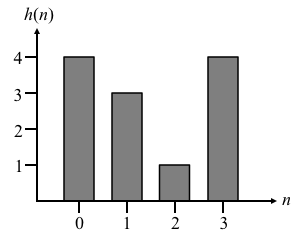
\includegraphics[width=.45\textwidth]{sampleHistogram} \label{sampleHist} }
\subfigure[Example 2-bpp Images with Identical Intensity Histograms (0 to 3 :: Black to White)]{ 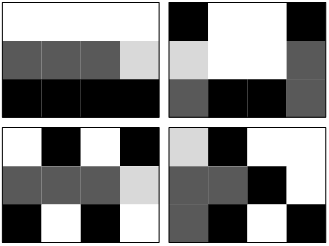
\includegraphics[width=.45\textwidth]{sampleImages} \label{sampleIm} }
\end{figure}

After understanding what a histogram is and how to build it, its use is only as good as its limitations. And one of the most important limitations of an intensity histogram is the loss of spatial information in its generation. No spatial information is mathematically present in the calculation of a basic intensity histogram, as it has been described and used herein. To illustrate this concept Figure \ref{sampleHist} displays a very simple histogram for a 2-bpp image of size $3\times4$. Figure \ref{sampleIm} shows 4 unique images that all share the histogram shown in Figure \ref{sampleHist}. These images come from the set of 138,600 possible images $\left(\frac{12!}{4!\cdot3!\cdot1!\cdot4!}\right)$ that share the histogram in Figure \ref{sampleHist}. But this is just a purely mathematical example with no constraints. By the nature of reality, such as the spatial and temporal continuity of objects within reality, images of real scenes are highly constrained subset of all the possible images from the total set (all the possible combinations of intensities given the number of pixels in the image). Any 2-bpp image of size $3\times4$ is actually in the general set of $4^{12}$ images, and so the set of images with the histogram in Figure \ref{sampleIm} is roughly less than $0.8\%$ of the total set, while still unconstrained to real world shapes. Extending this idea to the images used in this algorithm, which were all roughly of the size $480 \times 640$ and were 3 channel images of 8-bpp, that gives 768 possible values per pixel location ($3\cdot2^{8}$). This means that there are $768^{480\cdot640}$ possible images of this size with no spatial or histogram constraint. Any histogram, color constancy model, texture, object contiguity, or any other real world aspect or feature relevant to the digital image will create a smaller and smaller subset. It is thus applicable to determine that the approximation of using a normalized histogram to produce the PMF of an image is a theoretically relevant and an apt, realistic association. Conceptually what is being stated or assumed is that when viewing the same scene, two different views will be sampling the same random function, meaning that they should be describable by the same PMF in the overlap region, as that scene is relatively unique from the set of all possible digital images of that size and depth. As the overlap decreases between the views, the scene being captured is varying more and more, between the views, as parallax and occlusions begin to occur. The assumption that this is a small set of possible images since they are viewing the same scene is still valid; but the assertion that the views are still observing the same scene begins to fall apart. The PMFs of each view in the overlap as the cameras are rotated or separated by significant amounts become more independent and thus more separable and their possible mutual information decreases. It will be shown as a major characteristic of the evaluation of this algorithm and its robustness, to understand what factors and scenarios are crippling or limiting in terms of asserting dependence between the distinct views' PMFs. Also, As $\mathfrak{m}$ and $\mathfrak{n}$ decrease there is less opportunity for variation or consistency in the image, depending upon the value of $b$ (the bit-depth). If $2^{b}$ is significant (\ie not much, much less) compared to $\mathfrak{m} \cdot \mathfrak{n}$, then each instance of an image from that theoretical set can have significant variation. This could even allow for significant variation between views are capturing the same exact scene or sections of the views are capturing the same exact scene (spatio-temporally). This is a crippling limit of these assumptions and a source of our empirically understood minimum-overlap requirement for the algorithm.


%%%%%%%%%%%%%%%%%%%%%%%%%%%%%%%%%%%%%%%%%%%%%%%%%%%%%%%%%%%%%%%%%%%%%%%%%%%%%%%
% END OF DOCUMENT

